% GNUPLOT: LaTeX picture with Postscript
\begingroup
  \makeatletter
  \providecommand\color[2][]{%
    \GenericError{(gnuplot) \space\space\space\@spaces}{%
      Package color not loaded in conjunction with
      terminal option `colourtext'%
    }{See the gnuplot documentation for explanation.%
    }{Either use 'blacktext' in gnuplot or load the package
      color.sty in LaTeX.}%
    \renewcommand\color[2][]{}%
  }%
  \providecommand\includegraphics[2][]{%
    \GenericError{(gnuplot) \space\space\space\@spaces}{%
      Package graphicx or graphics not loaded%
    }{See the gnuplot documentation for explanation.%
    }{The gnuplot epslatex terminal needs graphicx.sty or graphics.sty.}%
    \renewcommand\includegraphics[2][]{}%
  }%
  \providecommand\rotatebox[2]{#2}%
  \@ifundefined{ifGPcolor}{%
    \newif\ifGPcolor
    \GPcolortrue
  }{}%
  \@ifundefined{ifGPblacktext}{%
    \newif\ifGPblacktext
    \GPblacktextfalse
  }{}%
  % define a \g@addto@macro without @ in the name:
  \let\gplgaddtomacro\g@addto@macro
  % define empty templates for all commands taking text:
  \gdef\gplbacktext{}%
  \gdef\gplfronttext{}%
  \makeatother
  \ifGPblacktext
    % no textcolor at all
    \def\colorrgb#1{}%
    \def\colorgray#1{}%
  \else
    % gray or color?
    \ifGPcolor
      \def\colorrgb#1{\color[rgb]{#1}}%
      \def\colorgray#1{\color[gray]{#1}}%
      \expandafter\def\csname LTw\endcsname{\color{white}}%
      \expandafter\def\csname LTb\endcsname{\color{black}}%
      \expandafter\def\csname LTa\endcsname{\color{black}}%
      \expandafter\def\csname LT0\endcsname{\color[rgb]{1,0,0}}%
      \expandafter\def\csname LT1\endcsname{\color[rgb]{0,1,0}}%
      \expandafter\def\csname LT2\endcsname{\color[rgb]{0,0,1}}%
      \expandafter\def\csname LT3\endcsname{\color[rgb]{1,0,1}}%
      \expandafter\def\csname LT4\endcsname{\color[rgb]{0,1,1}}%
      \expandafter\def\csname LT5\endcsname{\color[rgb]{1,1,0}}%
      \expandafter\def\csname LT6\endcsname{\color[rgb]{0,0,0}}%
      \expandafter\def\csname LT7\endcsname{\color[rgb]{1,0.3,0}}%
      \expandafter\def\csname LT8\endcsname{\color[rgb]{0.5,0.5,0.5}}%
    \else
      % gray
      \def\colorrgb#1{\color{black}}%
      \def\colorgray#1{\color[gray]{#1}}%
      \expandafter\def\csname LTw\endcsname{\color{white}}%
      \expandafter\def\csname LTb\endcsname{\color{black}}%
      \expandafter\def\csname LTa\endcsname{\color{black}}%
      \expandafter\def\csname LT0\endcsname{\color{black}}%
      \expandafter\def\csname LT1\endcsname{\color{black}}%
      \expandafter\def\csname LT2\endcsname{\color{black}}%
      \expandafter\def\csname LT3\endcsname{\color{black}}%
      \expandafter\def\csname LT4\endcsname{\color{black}}%
      \expandafter\def\csname LT5\endcsname{\color{black}}%
      \expandafter\def\csname LT6\endcsname{\color{black}}%
      \expandafter\def\csname LT7\endcsname{\color{black}}%
      \expandafter\def\csname LT8\endcsname{\color{black}}%
    \fi
  \fi
    \setlength{\unitlength}{0.0500bp}%
    \ifx\gptboxheight\undefined%
      \newlength{\gptboxheight}%
      \newlength{\gptboxwidth}%
      \newsavebox{\gptboxtext}%
    \fi%
    \setlength{\fboxrule}{0.5pt}%
    \setlength{\fboxsep}{1pt}%
\begin{picture}(7200.00,5040.00)%
    \gplgaddtomacro\gplbacktext{%
      \csname LTb\endcsname%
      \put(198,1320){\makebox(0,0)[r]{\strut{}}}%
      \put(198,1680){\makebox(0,0)[r]{\strut{}}}%
      \put(198,2040){\makebox(0,0)[r]{\strut{}}}%
      \put(198,2400){\makebox(0,0)[r]{\strut{}}}%
      \put(198,2760){\makebox(0,0)[r]{\strut{}}}%
      \put(198,3119){\makebox(0,0)[r]{\strut{}}}%
      \put(198,3479){\makebox(0,0)[r]{\strut{}}}%
      \put(198,3839){\makebox(0,0)[r]{\strut{}}}%
      \put(198,4199){\makebox(0,0)[r]{\strut{}}}%
      \put(735,1125){\rotatebox{45}{\makebox(0,0)[r]{\strut{}\tiny{\textrm{prazan/nedovr\v{s}en fajl}}}}}%
      \put(1139,1125){\rotatebox{45}{\makebox(0,0)[r]{\strut{}\tiny{\textrm{\texttt{scanf}/\texttt{printf} bez \texttt{cstdio}}}}}}%
      \put(1544,1125){\rotatebox{45}{\makebox(0,0)[r]{\strut{}\tiny{\textrm{nedeklarisana promenljiva}}}}}%
      \put(1948,1125){\rotatebox{45}{\makebox(0,0)[r]{\strut{}\tiny{\textrm{project file umesto sorsa}}}}}%
      \put(2353,1125){\rotatebox{45}{\makebox(0,0)[r]{\strut{}\tiny{\textrm{\texttt{scanf\_s}}}}}}%
      \put(2757,1125){\rotatebox{45}{\makebox(0,0)[r]{\strut{}\tiny{\textrm{\texttt{system("PAUSE")} bez \texttt{cstdlib}}}}}}%
      \put(3162,1125){\rotatebox{45}{\makebox(0,0)[r]{\strut{}\tiny{\textrm{\texttt{abs} bez \texttt{cstdlib}}}}}}%
      \put(3567,1125){\rotatebox{45}{\makebox(0,0)[r]{\strut{}\tiny{\textrm{
      \texttt{char == "\#"}}}}}}%
      \put(3971,1125){\rotatebox{45}{\makebox(0,0)[r]{\strut{}\tiny{\textrm{rezervisano ime promenljive}}}}}%
      \put(4376,1125){\rotatebox{45}{\makebox(0,0)[r]{\strut{}\tiny{\textrm{\texttt{iostream.h}}}}}}%
      \put(4780,1125){\rotatebox{45}{\makebox(0,0)[r]{\strut{}\tiny{\textrm{nema ;}}}}}%
      \put(5185,1125){\rotatebox{45}{\makebox(0,0)[r]{\strut{}\tiny{\textrm{\texttt{niz[][]}}}}}}%
      \put(5589,1125){\rotatebox{45}{\makebox(0,0)[r]{\strut{}\tiny{\textrm{dodela vrednosti nizu}}}}}%
      \put(5994,1125){\rotatebox{45}{\makebox(0,0)[r]{\strut{}\tiny{\textrm{\} vi\v{s}ka}}}}}%
      \put(6398,1125){\rotatebox{45}{\makebox(0,0)[r]{\strut{}\tiny{\textrm{\texttt{std::sort} bez \texttt{algorithm}}}}}}%
    }%
    \gplgaddtomacro\gplfronttext{%
      \csname LTb\endcsname%
      \put(3566,4709){\makebox(0,0){\strut{} \textrm{\textbf{Compile error}}}}%
    }%
    \gplbacktext
    \put(0,0){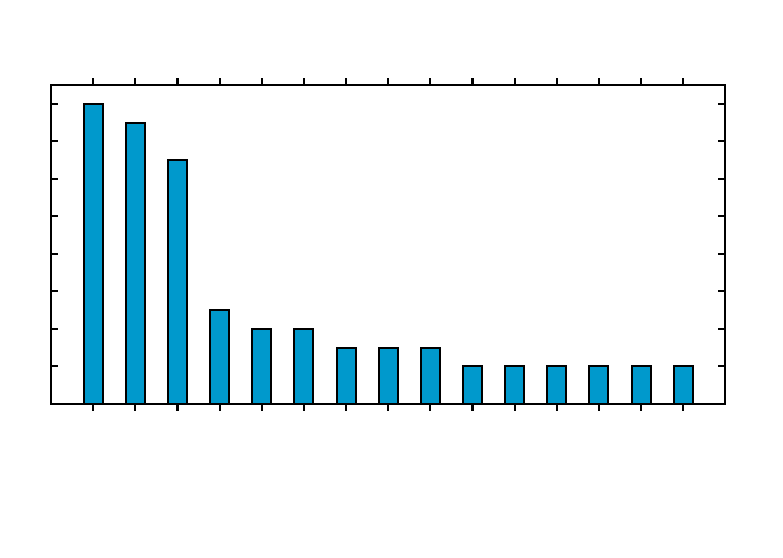
\includegraphics{figs/ceokr}}%
    \gplfronttext
  \end{picture}%
\endgroup
